%%=========================================
\chapter{Theoretical Background}
\label{chp:theory}
\begin{info}
	Within this 'info' environment you can write stuff you don't want to be included in the final version of the report
\end{info}

In the theoretical background, I will start by introducing the different datasources that serves as input to Vake's pipline. A big part of this project is to understand the data, in order to know what to do with it later on.
Next up, I will explain how Vake uses this data to create a pipeline for ship detection. This will be useful for understanding how to scope my project later on. 
The last part of the theoretical background will contain some state-of-the-art modelling of AIS-predictions and reconstruction. This will help me to understand where the technology is today, and how I can apply general solutions to my specific challenge. 
%%-----------------------------------------
\section{Automatic Identification System (AIS)}
\begin{info}{}
	
\end{info}
%%-----------------------------------------
AIS is a large integrated system that combines equipment and protocols to send, recieve and decode navigational information from ships at sea. There are landmounted receivers, satelitte receivers and ship-mounted transcievers that constantly sends, receives and utilizes this information to improve maritime security and enhance monitoring, among other things.

According to the International Maritime Organization (IMO) \cite{MarineSafteyComittee}, the transcievers mounted on the individual ships must provide identity, ship-type, position, course, speed, and other safety-related information. 
The requlation enforced by IMO in 2002 also states that all ships of 300 gross tonnage or above engaging on international voyages, as well as all cargo ships above 500 gross tonnage and all passenger ships must be equipped with such technology. 

The global adaption of AIS has lead to an incredible amount of data with a large number of use-cases not imagined when IMO first enforced the system.   

\todo[inline]{List use cases for AIS. mabye find the source where IMO regretted public AIS-data}


\todo[inline]{Sub-chapters: How AIS works}
\todo[inline]{Sub-chapters: Protocol}
\todo[inline]{Sub-chapters: Weaknesses}


%%=========================================

%------------------------------------------
\section{Sentinel-2 mission}
\begin{info}{}
	A quick introduction to what Sentinel-2 data is. 
	I need to talk about the postprocessing that leads to MGRS-tiles.  
\end{info}
%%-----------------------------------------
The Copernicus Sentinel-2 mission is a constellation of two orbiting satellites, aiming to monitor variability in land surface conditions. \cite{EuropeanSpaceAgency}
The satellites achieve this by global acquisitions of high-resolution multispectral images with a high revisit frequency.

To create these images, the satelittes has an onboard Multi-Spectral Instrument (MSI) that creates images with 13 spectral bands. To capture these images, the sensor uses a push-broom technique that takes in rows of data. Such a datatake is then further processed and made publicily available for download. 

One of the products that is available for download is called Level-1C. The raw data undergoes many steps before becoming Level-1C, with compression and refinement of the physical geometric model using ground control points being major steps of interest. lastly, the data is orthorectified and cut into tiles. These tiles are of 100km x 100km in the UTM/WGS84 projection.

\section{Military Grid Reference System}
\begin{info}{}

\end{info}
%%-----------------------------------------

One of the findings in \cite{Tofting2018} is that the tiles from the Sentinel-2 Level-1C product corresponds to the Military Grid Reference System (MGRS). The MGRS is used by NATO, being derived from the Universal Polar Stereographic(UPS)- and the Universal Transverse Mercator (UTM)-projections. This system does not define points, but rather an area on a map. 

In MGRS, the world is divided into 6 by 8 degrees geographic areas, each is given an unique identifier called the Grid Zone Designation (GZD). \cite{NationalGeospatial-IntelligenceAgency2014} The GZD is an alphanumeric code starting with the zone number from either UTM (80° south to 84° north) or UPS. The next element is a letter that defines the lattitude bond. Beginning at 80° south and proceeding northward, twenty bands are lettered C through X, omitting I and O. The bands are 8 degrees wide. Within each o f the GZD's, these large tiles are divided into a grid consisting of smaller 100km x 100km tiles. These tiles are indexed by two more letters, indicating the specific row and column within the GZD. It is these smaller tiles within the GZD's that corresponds with the Level-1C products. This creates consistent zones for the images produced by the satellites.



\section{AIS Data Management}
\begin{info}{}
	This is a simple section saved in a separate file.
\end{info}
%%-----------------------------------------

\section{Vake's AIS Fuser}
\begin{info}{}
	This is a simple section saved in a separate file.
\end{info}
%%-----------------------------------------
Vake has implemented a fuser that uses different methods for predicting the position of a ship at the time of the captured image. Their general outline is structured in the following way. 


\begin{enumerate}
	\item The fuser takes in the finished products with image detections from the detection model. These products are on a tabular format, and the two values used in the fuser is the sensing time and image footprint. 
	\item The next step is to extract all AIS data within the image timestamp. In order to lower the amount of data, the algorithm takes a threshold value. 
	\item Further filtering the data, all AIS messages outside the image footprint is discarded. Also here we use a buffer, the default is 5000 meters. This is to include those ships that are just leaving or just entering the footprint. 
	\item Using the aqcuired AIS-messages, the last prior and the first posterior is selected, based on the product timestamp. 
	\item Next, interpolation parameters are generated, taking into consideration the different edge cases that can cause problems. When the time difference between the signals are 0, the interpolated speed is set to 0.
	
	If the speeds reported in the AIS messages are invalid, the interpolated speed is calculated using the mean speed between the points. $d_x/d_t$ Otherwise it is calculated by $speed_{interpolated} = speed_{prior}*0.514444444 + d_v/d_t * d_{ti}$

	\item They do something similar on the interpolation of the distance travelled where $distance=((speed_{prior}*0.514444444 + speed_{calc})/2)*d_{ti}$ 
	In addition, the distance using the mean speed is calculated.
	
	\item next multiple extrapolations and interpolations is calculated. We can list interpolatedGeom, meanInterpolatedGeom, priorExtrapolatedGeom,  pastExtrapolatedGeom. 
	\item These calculations, along with the MMSI is joined on other static AIS data and returned for further processing. The interpolations are sent into what Vake calls the "LikelyLocationDecisionTree" as we can see in figure \ref{fig:decisiontree}. This decision tree desides which interpolation method should be used to calculate the final estimated ship position. The decision tree exists because the characteristics of the interpolation is highly dependent on when the prior and posterios messages are sampled from. If they are far away from eachother, the heading is varying to much, or not a part of a straight line, this will affect the precision of the different methods. In the end, the selected method result is returned for that particular ship
	\item the final step is to do a nearest neighbour-search between the different detections with a given threshold, matching the interpolated positions to the detections if the distance is close enough for it to be a match.   
	\todo[inline]{Explain the speed = 0 and cite why temporal before spatial filtering}
	\todo[inline]{Should i specify what the different steps does?}
\end{enumerate}	

\begin{figure}[h]
	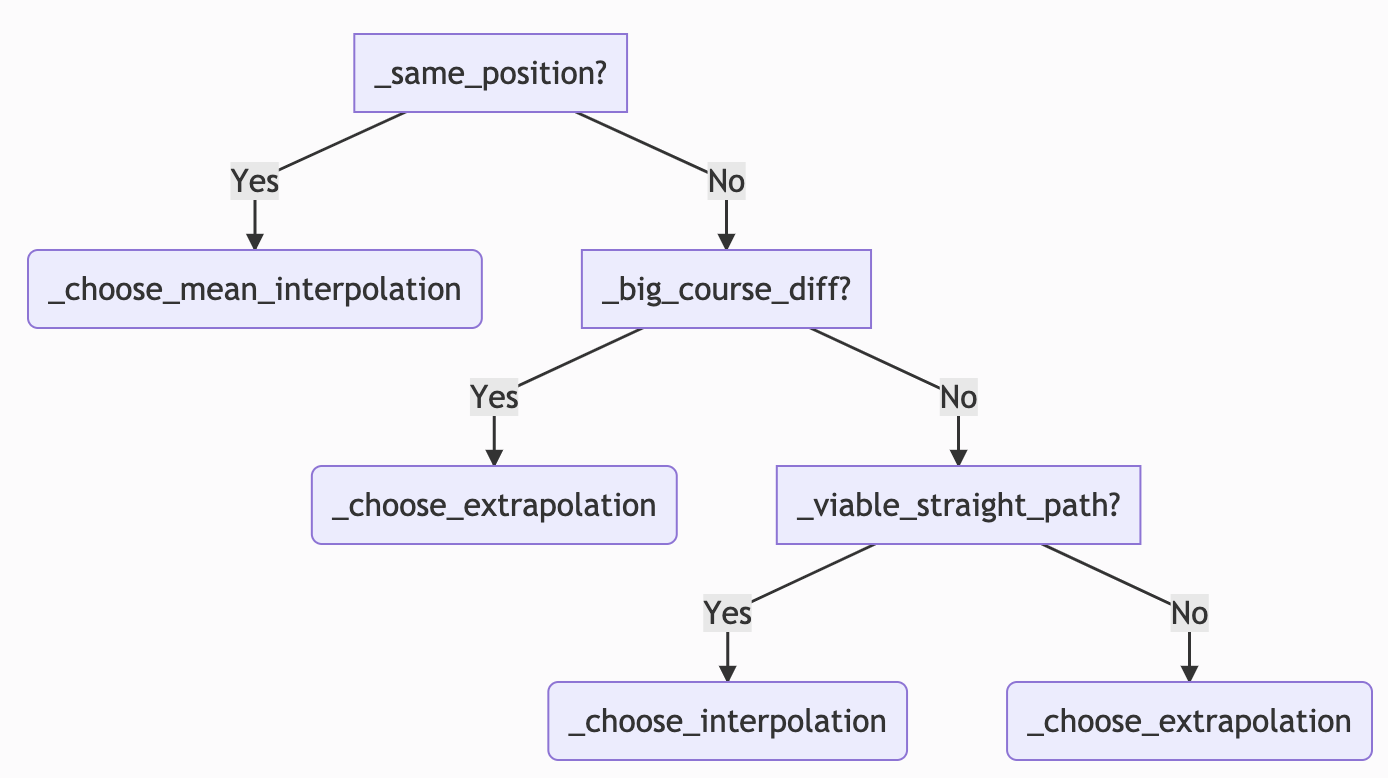
\includegraphics[scale=0.2]{likelylocationdecisiontree.png}
	\centering
	\caption{Vake's decision tree for selecting interpolation methods,  }
	\centering
	\label{fig:decisiontree}
\end{figure}

\subsection{Fuser weaknesses}
%%-----------------------------------------
\begin{enumerate}
	\item Not a probabilistic model, it either gives a binary match, or no match at all. There is no quantified figure for how accurate or how sure the interpolator thinks it is. 
	\item The fuser only considers the prior and posterior signal with regards to the sensing time, this excludes a lot of data which could have been used to better understand the ship-movement. 
	\item It is very sensitive to signal blackout and poorer resolution which leads to larger gaps in the data coverage. The assumption that simple interpolation works is weakened when the ships travel over large distances without reporting their position. 
	\item The interpolation/extrapolation is a linear model, unable to handle the natural curvilinear motion of ships. The theory is that it is not expressive enough to capture all ship-behaviour. 
	\item The thresholds for the decision tree is created through trial and error and is not tested for efficiency or accuracy.
	\item The model for interpolating does not take into account the actual detections, it only tries to match after the interpolation is done. This is and an important datasource to optimize for. 
\end{enumerate}	


%%=========================================

%%=========================================

%%=========================================
\section{Current research on AIS-preprocessing}
\begin{info}{}
	This is a simple section saved in a separate file.
\end{info}
%%-----------------------------------------




%%=========================================

%%=========================================
\section{Current research on AIS-predictions and -reconstruction}
\begin{info}{}
	This is a simple section saved in a separate file.
\end{info}
%%-----------------------------------------





%%=========================================


%%=========================================